\chapter{Backtesting Strategies}
\label{ch:backtest}

\begin{companioncode}{qf-05-backtest}
Code: \texttt{crates/qf-05-backtest/}\\
Dependencies: \crate{qf-common}, \crate{qf-03-stocks}, \crate{qf-04-returns}\\
Run: \texttt{cargo run -p qf-05-backtest --example backtest\_demo}
\end{companioncode}

\section{Learning Objectives}

This chapter introduces the mechanics of evaluating a trading strategy on
historical data. After completing it you can:

\begin{itemize}
    \item Explain what a backtest is --- and what it is not
    \item Generate trading signals from indicators with no look-ahead bias
    \item Account for transaction costs in P\&L
    \item Evaluate a strategy with the risk-adjusted metrics from
      \cref{ch:returns}
    \item Avoid the three classic backtest traps: overfitting, look-ahead
      bias, and survivorship bias
\end{itemize}

\begin{keyinsight}
A backtest is a \emph{simulation}, not a prediction. It tells you how a
strategy \emph{would have} performed, not how it \emph{will} perform. The number
one failure mode is overfitting to historical data: a strategy that looks
great in backtest and loses money in production.
\end{keyinsight}

\section{What Is Backtesting?}

Backtesting is the replay of a trading strategy over historical price data,
bar by bar, to estimate its hypothetical performance. The engine maintains
state (position, cash, equity) and lets the strategy decide, at each bar,
what action to take given the price history it has seen so far.

\marginnote{%
\textbf{Simulation vs prediction}\\[0.3em]
A backtest does not predict. It is a \emph{counterfactual}: ``if you had
traded this strategy with these rules in this market, here is what would have
happened.'' Any conclusion about the future requires additional assumptions
(market stationarity, capacity, regime persistence) that the backtest itself
cannot validate.
}

Three assumptions are implicit and worth naming:

\begin{enumerate}
    \item \textbf{Market stationarity}: the statistical properties of the
      historical sample are representative of the future. Often false.
    \item \textbf{Capacity}: the strategy can take the simulated sizes without
      moving the market. True for retail; false for institutional size.
    \item \textbf{Execution}: the simulated fills are achievable. Slippage,
      partial fills, and market impact are real and cost money.
\end{enumerate}

\section{Signals and Positions}

\marginnote{%
\textbf{Signal vs position}\\[0.3em]
A signal is an \emph{instruction} (what to do this bar); a position is
a \emph{state} (what we are currently holding). The engine applies the
signal to update the position. Decoupling them lets you replay the
same signal stream under different execution models.
}

A \emph{signal} is a discrete instruction for the current bar. We use three:

\begin{lstlisting}[language=Rust]
#[derive(Debug, Clone, Copy, PartialEq, Eq)]
pub enum Signal {
    Buy,  // Enter long
    Sell, // Exit long (long-only for this chapter)
    Hold, // Do nothing
}
\end{lstlisting}

A \emph{position} is what the engine is currently holding:

\begin{lstlisting}[language=Rust]
#[derive(Debug, Clone, Copy, PartialEq, Eq)]
pub enum Position {
    Long,  // Holding the asset
    Short, // Reserved for later phases
    Flat,  // No position
}
\end{lstlisting}

\begin{keyinsight}
Why separate \texttt{Signal} and \texttt{Position}? A signal is an
\emph{intention}; a position is a \emph{state}. The engine translates
intentions into state transitions, charging transaction costs on every
change. This separation lets the strategy stay declarative (``I want to be
long now'') and the engine stay responsible for the messy realities
(costs, fill assumptions, position limits).
\end{keyinsight}

\section{The Strategy Trait}

\marginnote{%
\textbf{No look-ahead}\\[0.3em]
\texttt{signal(data, index)} receives \texttt{data[..=index]}. The strategy
must never read past the current bar. The engine enforces this by passing a
slice and the current index --- implementations physically cannot access
\texttt{data[index+1..]} without unsafe code.
}

The extension point of the engine is the \texttt{Strategy} trait:

\begin{lstlisting}[language=Rust]
pub trait Strategy {
    fn signal(&self, data: &[Ohlcv], index: usize) -> Signal;
    fn name(&self) -> &str;
}
\end{lstlisting}

The engine is generic over \texttt{S: Strategy}, so new strategies drop in
without engine changes. The trait takes the full slice plus the current index
so the strategy can compute any indicator that fits in the observed history.

\section{SMA Crossover}

The canonical first strategy: go long when a short moving average crosses
above a long moving average (the \emph{golden cross}); exit when it crosses
below (the \emph{death cross}).

\marginnote{%
\textbf{Golden / death cross}\\[0.3em]
$\text{SMA}_S$ crosses above $\text{SMA}_L$ $\Rightarrow$ Buy\\[0.3em]
$\text{SMA}_S$ crosses below $\text{SMA}_L$ $\Rightarrow$ Sell\\[0.5em]
A crossover is a \emph{change in the relationship}, not a level. The previous
bar must satisfy the opposite inequality.
}

\begin{lstlisting}[language=Rust]
pub struct SmaCrossover {
    short_period: usize,
    long_period: usize,
}

impl Strategy for SmaCrossover {
    fn signal(&self, data: &[Ohlcv], index: usize) -> Signal {
        if index < self.long_period { return Signal::Hold; }

        let short_now = match sma_at(data, index, self.short_period) {
            Some(v) => v, None => return Signal::Hold,
        };
        let long_now = match sma_at(data, index, self.long_period) {
            Some(v) => v, None => return Signal::Hold,
        };
        let short_prev = match sma_at(data, index - 1, self.short_period) {
            Some(v) => v, None => return Signal::Hold,
        };
        let long_prev = match sma_at(data, index - 1, self.long_period) {
            Some(v) => v, None => return Signal::Hold,
        };

        let crossed_up   = short_prev <= long_prev  && short_now >  long_now;
        let crossed_down = short_prev >= long_prev  && short_now <  long_now;

        if crossed_up   { Signal::Buy  }
        else if crossed_down { Signal::Sell }
        else { Signal::Hold }
    }
    fn name(&self) -> &str { "SMA Crossover" }
}
\end{lstlisting}

\begin{keyinsight}
Crossover strategies are \emph{trend followers}: they only make money when
prices trend. In choppy, mean-reverting markets they lose, because each
crossover is a false signal that gets reversed at the next crossover --- with
transaction costs paid on both sides.
\end{keyinsight}

\section{P\&L with Transaction Costs}

\marginnote{%
\textbf{Transaction cost}\\[0.3em]
At entry: $c_{\text{entry}} = \text{notional} \cdot \tau$\\[0.3em]
At exit: $c_{\text{exit}} = \text{shares} \cdot P_{\text{exit}} \cdot \tau$\\[0.5em]
Net P\&L: $\text{shares} \cdot (P_{\text{exit}} - P_{\text{entry}}) - c_{\text{entry}} - c_{\text{exit}}$
}

Every state change costs money. The engine charges a proportional cost
$\tau$ (e.g.\ $\tau = 0.001$ for 10 basis points) on the traded notional:

\begin{lstlisting}[language=Rust]
// Enter long: spend all cash at the close, paying the cost first.
let notional = capital;
let cost = notional * config.transaction_cost;
shares = (notional - cost) / price;
total_costs += cost;

// Exit long: sell all shares at the close.
let notional = shares * price;
let cost = notional * config.transaction_cost;
total_costs += cost;
capital = notional - cost;
\end{lstlisting}

At each bar, equity is marked to market: \texttt{shares * close} when long,
cash when flat. The per-bar simple returns of the equity curve become the
\texttt{daily\_returns} used by the risk metrics from \cref{ch:returns}.

\section{Performance Evaluation}

\marginnote{%
\textbf{Why reuse \crate{qf-04-returns}?}\\[0.3em]
Sharpe, Sortino, and max drawdown are return-level statistics --- they
do not care how the returns were generated. Once the backtest produces
a daily return series, evaluation is identical to computing the same
metrics on a buy-and-hold benchmark. Code reuse follows the math.
}

\texttt{BacktestResult} delegates to \texttt{qf-04-returns} for the four
headline metrics:

\begin{lstlisting}[language=Rust]
impl BacktestResult {
    pub fn sharpe(&self, rf: f64) -> f64 {
        qf_04_returns::annualized_sharpe(&self.daily_returns, rf, 252.0)
    }
    pub fn sortino(&self, rf: f64) -> f64 {
        qf_04_returns::sortino_ratio(&self.daily_returns, rf)
    }
    pub fn max_drawdown(&self) -> f64 {
        qf_04_returns::max_drawdown(&self.equity_curve)
    }
    pub fn volatility(&self) -> f64 {
        qf_04_returns::annualized_volatility(&self.daily_returns, 252.0)
    }
}
\end{lstlisting}

\begin{keyinsight}
The risk metrics operate on the \emph{equity curve}, not the raw price
series. A strategy that goes flat for half the period has a different risk
profile from buy-and-hold even on the same underlying, because the equity
curve is flat whenever the position is flat. Volatility and drawdown reflect
this exposure pattern automatically.
\end{keyinsight}

\section{Buy-and-Hold Benchmark}

\marginnote{%
\textbf{Always compare to buy-and-hold}\\[0.3em]
An active strategy that returns $10\%$ looks good until you realise
the underlying asset returned $15\%$ over the same period. The
buy-and-hold benchmark is the floor any active strategy must beat
\emph{after} costs. If it does not, the activity added no value.
}

Every active strategy must be compared against the simplest alternative: buy
on the first bar and hold forever. \texttt{BuyAndHold} is a two-line strategy:

\begin{lstlisting}[language=Rust]
impl Strategy for BuyAndHold {
    fn signal(&self, _data: &[Ohlcv], index: usize) -> Signal {
        if index == 0 { Signal::Buy } else { Signal::Hold }
    }
    fn name(&self) -> &str { "Buy and Hold" }
}
\end{lstlisting}

If an active strategy cannot beat buy-and-hold after costs, the active
component is adding noise and cost, not value. The benchmark also lets you
decompose returns: alpha (skill) vs beta (market exposure).

\section{Common Pitfalls}

\marginnote{%
\textbf{The two cardinal sins}\\[0.3em]
\emph{Overfitting} and \emph{look-ahead bias} are the two ways a
backtest lies to you. Overfitting makes the past look good; look-ahead
bias makes the future knowable. Both produce strategies that fail
miserably in live trading. Treat any backtest Sharpe $> 2$ with deep
suspicion until both are ruled out.
}

\begin{description}
    \item[Overfitting] Tuning the SMA periods $(S, L)$ to maximise in-sample
      Sharpe almost always produces a strategy that fails out-of-sample. Use
      walk-forward validation (deferred to a later phase) and be suspicious of
      parameters tuned on the same data you evaluate on.
    \item[Look-ahead bias] Using information not available at decision time.
      Common sources: using the close of bar $t$ to decide at bar $t$ (only
      valid if the trade executes at the close), indicator warm-up that reads
      the future, corporate actions applied with hindsight. Our
      \texttt{signal(data, index)} interface rules out most of these by
      construction.
    \item[Survivorship bias] Backtesting only on companies that survived to the
      present. Companies that went bankrupt are absent, inflating historical
      returns. Use point-in-time universes when available.
\end{description}

\section{Example Output}

\begin{lstlisting}[language=bash]
$ cargo run -p qf-05-backtest --example backtest_demo
==============================
Backtest Results
==============================

Period: 2024-001 to 2024-252

--- Strategy: SMA Crossover (10/30) ---
  Total Return:   3.49%
  Sharpe (ann.):   2.55
  Sortino:         0.31
  Max Drawdown:    -0.41%
  Trades:          1

--- Strategy: Buy and Hold ---
  Total Return:    4.54%
  Sharpe (ann.):   1.70
  Max Drawdown:    -6.35%

Outperformance vs Buy & Hold: -1.04%
\end{lstlisting}

The SMA crossover underperforms buy-and-hold in this synthetic regime: the
cost of false signals in choppy sections outweighs the benefit of avoiding
the mid-year drawdown. This is the typical result for trend-following
strategies in noisy markets, and it is the right lesson to take from a first
backtest.

\section{Walk-Forward Analysis}
\label{sec:walk-forward}

\marginnote{%
\textbf{Walk-forward vs k-fold}\\[0.3em]
Unlike k-fold CV (which can use future data in some folds),
walk-forward strictly respects time ordering. Each window trains
on past data and tests on subsequent data --- mimicking real trading.
}

Walk-forward analysis addresses the overfitting trap by enforcing a strict
temporal separation between training and testing windows. Instead of tuning
parameters on the full dataset and evaluating on the same data, walk-forward
splits the time series into sequential windows:

\begin{enumerate}
    \item \textbf{In-sample window}: Historical data used for parameter tuning
    \item \textbf{Out-of-sample window}: Future data (not seen during tuning) for evaluation
    \item \textbf{Rolling forward}: Advance both windows and repeat
\end{enumerate}

\subsection{Walk-Forward Efficiency}

\marginnote{%
\textbf{Interpreting WFE}\\[0.3em]
$\text{WFE} = 1.0$: Strategy performs equally well in-sample and out-of-sample (ideal)\\[0.3em]
$\text{WFE} > 1.0$: Strategy performs \emph{better} out-of-sample (rare, check for bugs)\\[0.3em]
$\text{WFE} \approx 0.5$: Typical degradation for robust strategies\\[0.3em]
$\text{WFE} < 0.3$: Severe overfitting --- strategy likely fails in live trading
}

Walk-Forward Efficiency (WFE) quantifies how much performance degrades from
in-sample to out-of-sample:

\begin{equation}
\text{WFE} = \frac{\text{Sharpe}_{\text{out-of-sample}}}{\text{Sharpe}_{\text{in-sample}}}
\end{equation}

A WFE close to 1.0 indicates a robust strategy; values below 0.5 suggest
severe overfitting. The ratio measures how much ``alpha'' survived the
transition from tuning to live-like conditions.

\subsection{Implementation}

The \texttt{quant-backtest} crate provides walk-forward support via the
\texttt{WalkForward} cross-validator (see \cref{ch:afml} for
comprehensive AFML pipeline integration):

\begin{lstlisting}[language=Rust]
use quant_backtest::{WalkForward, WalkForwardConfig};
use quant_core::CrossValidator;

// Configure rolling 60-bar training, 20-bar testing, step 20 bars
let config = WalkForwardConfig::rolling(60, 20, 20);
let wf = WalkForward::new(config);

// Generate splits for 200 bars
let splits = wf.splits(0, 200);
// Returns: [ [0-60,60-80], [20-80,80-100], [40-100,100-120], ... ]
\end{lstlisting}

For each split: tune parameters on the in-sample window, freeze them, evaluate
on out-of-sample. Aggregate the out-of-sample Sharpe ratios and compute WFE.

\subsection{Visual Representation}

\begin{figure}[htbp]
\centering
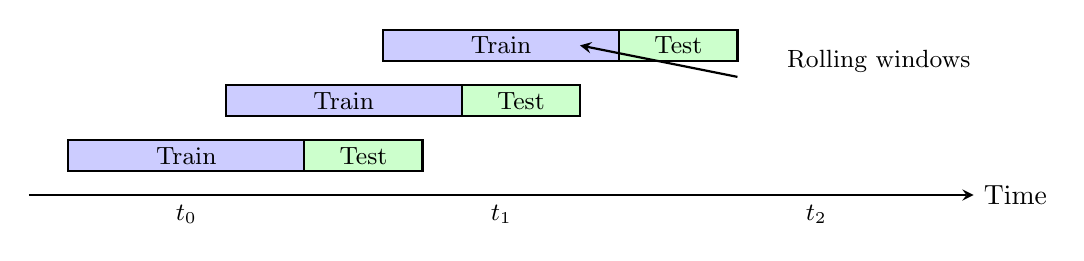
\begin{tikzpicture}[>=stealth, thick]
  % Timeline
  \draw[->] (0,0) -- (12,0) node[right] {Time};

  % Window 1
  \draw[fill=blue!20] (0.5,0.3) rectangle (3.5,0.7) node[midway] {\small Train};
  \draw[fill=green!20] (3.5,0.3) rectangle (5,0.7) node[midway] {\small Test};

  % Window 2
  \draw[fill=blue!20] (2.5,1.0) rectangle (5.5,1.4) node[midway] {\small Train};
  \draw[fill=green!20] (5.5,1.0) rectangle (7,1.4) node[midway] {\small Test};

  % Window 3
  \draw[fill=blue!20] (4.5,1.7) rectangle (7.5,2.1) node[midway] {\small Train};
  \draw[fill=green!20] (7.5,1.7) rectangle (9,2.1) node[midway] {\small Test};

  % Labels
  \node[below] at (2,0) {\small $t_0$};
  \node[below] at (6,0) {\small $t_1$};
  \node[below] at (10,0) {\small $t_2$};

  % Legend
  \node[right] at (9.5,1.7) {\small Rolling windows};
  \draw[->] (9,1.5) -- (7,1.9);
\end{tikzpicture}
\caption{Walk-forward rolling windows: each training window slides forward,
  testing on the next unseen period. Unlike k-fold, every test window is
  strictly after its training window.}
\label{fig:walk-forward}
\end{figure}

\subsection{Anchored vs Rolling}

\marginnote{%
\textbf{Trade-off}\\[0.3em]
\emph{Anchored}: More data, but older data may be stale\\[0.3em]
\emph{Rolling}: Fresher data, but smaller sample size
}

\begin{itemize}
    \item \textbf{Rolling window}: Training window slides (fixed size, moves forward)
      \begin{itemize}
        \item Advantages: Uses only recent data (regime-aware)
        \item Disadvantages: Smaller training sets, higher variance
      \end{itemize}

    \item \textbf{Anchored window}: Training window expands (grows over time)
      \begin{itemize}
        \item Advantages: Larger training sets, lower variance
        \item Disadvantages: Older data may represent outdated regimes
      \end{itemize}
\end{itemize}

Choose rolling for high-frequency or regime-sensitive strategies; choose
anchored for slower, more stable strategies.

\begin{keyinsight}
Walk-forward analysis is the \emph{minimum viable safeguard} against
overfitting. It does not eliminate overfitting (you can still overfit
by cherry-picking the best split or tuning on WFE itself), but it forces
the strategy to prove it can perform on unseen data. A strategy with
$\text{WFE} > 0.7$ is far more credible than one evaluated only in-sample.
\end{keyinsight}

For advanced walk-forward workflows integrated with AFML labeling, purged
k-fold, and bet sizing, see \cref{ch:afml}.

\section{Exercises}

\begin{enumerate}
    \item \textbf{Cost sensitivity}: Run the 10/30 crossover on the synthetic
      series for $\tau \in \{0, 0.001, 0.0025, 0.005, 0.01\}$. Plot total
      return vs $\tau$. At what cost does the strategy stop being profitable?

    \item \textbf{Parameter sensitivity}: For $\tau = 0.001$, sweep
      $(S, L) \in \{5, 10, 20\} \times \{30, 50, 100\}$ with $S < L$. Which
      configuration maximises Sharpe? Is it the same one that maximises total
      return? Why or why not?

    \item \textbf{EMA crossover}: Implement an EMA crossover strategy by
      replacing SMA with \func{qf\_03\_stocks::ema}. Compare its turnover
      (number of trades) and Sharpe against the SMA crossover on the same
      data.

    \item \textbf{Position sizing}: Modify the engine to invest a fixed
      fraction $f \in (0, 1]$ of capital on each entry instead of 100\%.
      How does the equity curve change for $f = 0.5$? What is the trade-off?

    \item \textbf{Walk-forward (conceptual)}: Split the 252-bar series into
      an in-sample window (first 180 bars) and an out-of-sample window (last
      72 bars). Tune $(S, L)$ on the in-sample, freeze it, and evaluate on
      out-of-sample. How much does Sharpe degrade from in-sample to
      out-of-sample? This is the simplest walk-forward analysis.
\end{enumerate}

\section{Key Takeaways}

\begin{itemize}
    \item \textbf{Backtesting} is a simulation, not a prediction---it tells you
      how a strategy \emph{would have} performed
    \item \textbf{Signals vs positions}: signals are intentions, positions are
      state; the engine translates one to the other
    \item \textbf{Transaction costs} erode returns and must be modelled
      explicitly
    \item \textbf{SMA crossover} is a trend-following strategy that loses in
      choppy markets
    \item \textbf{Buy-and-hold} is the benchmark every active strategy must beat
    \item \textbf{Pitfalls}: overfitting, look-ahead bias, and survivorship bias
      are the classic backtest traps
\end{itemize}

\vspace{1em}
\noindent\textbf{Next chapter}: Foundations---moments, hand-rolled RNG, and
geometric Brownian motion simulation.